% CABECERA DESCRIPCIÓN
% BEGIN_FOLD
%%%%%%%%%%%%%%
% Fichero: uclmTFGesi.tex
% Autor: Jesús Salido Tercero (https://www.esi.uclm.es/www/jsalido)
% Fecha (creación): febrero 2010 
% Rev. : marzo 2024
% Descripción: Plantilla para memoria de TFG 
% (Escuela Sup. de Informática, UCLM). Creada para el curso 
% “LaTeX esencial para preparación de TFG, Tesis y otros documentos 
% académicos” (Esc. Sup. Informática-UCLM)
%
%### Compilación 
%
% Esta plantilla ha sido preparada para compilarse con `pdflatex`  
% (bibliografía con `bibtex`).
%$ $
% Para su compilación se aconseja utilizar `latexmk` (requiere para su 
% ejecución de un intérprete perl:
%
%> \$> latexmk -gg -pdf -bibtex-cond1 -quiet -outdir=build uclmTFGesi.tex
%
% Para la automatización del trabajo con esta plantilla es recomendable el 
% empleo de IDE dedicados como [TeXstudio](https://www.texstudio.org/).
%
% Una versión revisada de esta plantilla está disponible en overleaf.
% Puede crearse un proyecto propio para escribir un TFG directamente en 
% overleaf, o bien descargarla como un archivo .zip para su utilización en 
% modo local.
%
% Si deseas acceder a la versión de desarrollo puedes encontrarla en GitHub:
%	https://github.com/JesusSalido/TFG_ESI_UCLM
%%%%%%%%%%%%%%
% END_FOLD
\documentclass[final, % final o drafts (sin figuras)
			   spanish, % Español o inglés (english) como idioma pral. 
			   pageonfooter=false % Paginación en el pie
]{TFGesi}

% -------------------------
% EDITA: Datos del documento. 
% -------------------------
\tituloPrimera{Plantilla guía de TFG para la ESI-UCLM} % 1ª Línea
\tituloSegunda{Curso de {\LaTeX{}} esencial} % OPT.: Títulos largos.
\tituloCorto{Plantilla guía de TFG} % Título corto (mostrado en pág. de 
%créditos)
\autor{Jesús Salido Tercero}
\email{jesus.salido@uclm.es}					
\instEdu{UNIVERSIDAD DE CASTILLA-LA MANCHA}
\centroEdu{ESCUELA SUPERIOR DE INFORMÁTICA}
\titulacion{GRADO EN INGENIERÍA INFORMÁTICA}
\especialidad{Intensificación cursada}
\depto{Depto. del tutor(a)}
% (EN: BACHELOR IN COMPUTING ENGINEERING)
\tipoDoc{TRABAJO FIN DE GRADO} % (EN: BACHELOR DISSERTATION)
% Si las fechas se desean en inglés hay que ponerla explícita.
\mesTF{julio}        	% Mes de defensa
\monthTF{July}        	% En inglés
\yearTF{2024}        	% Año de defensa
\cityTF{Ciudad Real}	% Ciudad de defensa
\escudo{esiLogo}        % Logo centro (pdf, png o jpg)
% -------------------------

% Palabras clave: Son importantes para facilitar búsqueda en Internet
\setkeywords{%
	Escuela Superior de Informática, %
	Trabajo Fin de Grado, %
	\LaTeX, %
	plantilla de TFG, %
	UCLM %
} % (como mucho 5)

% -------------------------
% CUERPO del documento
% -------------------------
\begin{document}
\frontmatter
%\input{./Anexos/PortadaETSII} % Por ej.,: Otras portadas
%\includepdf{fichero_portada.pdf} % Incluso como fichero PDF

% -------------------------------------------------------------------------
% PORTADA PRAL. (1)
% -------------------------------------------------------------------------

%\portadaOld % Portada pral.
\portadaNew

% -------------------------------------------------------------------------
% PORTADA INTERIOR (2)
% -------------------------------------------------------------------------
\portadaInt %Portada interior


% -------------------------
% CRÉDITOS
% -------------------------
\begin{creditos}[\titulo] % Editar a conveniencia (se pasa el título deseado)
El autor puede elegir el tipo de licencia que desee. Este documento se distribuye con licencia CC BY-NC-SA 4.0. El texto completo de la licencia se puede obtener en \url{https://creativecommons.org/licenses/by-nc-sa/4.0/}. La copia y distribución de esta obra está permitida en todo el mundo, sin regalías y por cualquier medio, siempre que esta nota sea preservada. Se concede permiso para copiar y distribuir traducciones de este libro desde el español original a otro idioma, siempre que la traducción sea aprobada por el autor del libro y tanto el aviso de copyright como esta nota de permiso, sean preservados en todas las copias.

\noindent 
\includegraphics[width=0.15\linewidth]{by-nc-sa}

% Para citar este plantilla empleando bibtex puedes emplear el registro siguiente:
%@www{salidoTFG,
%  author       = {Jesús Salido},
%  title        = {Plantilla guía de TFG para la ESI-UCLM},
%  year         = {2019},
%  editor       = {GitHub},
%  organization = {Universidad de Castilla-La Mancha},
%  url          = {https://github.com/JesusSalido/TFG_ESI_UCLM},
%  doi          = {10.5281/zenodo.4574562}
%}
\end{creditos}


% -------------------------
% CALIFICACIÓN DEL TRIBUNAL  (No necesario en versión electrónica)
% -------------------------
%\tribunal % Página opcional para calificación 


% -------------------------
% DEDICATORIA 
% -------------------------
\begin{dedicatoria} % (no confundir con los agradecimientos)
\emph{A mis estudiantes \\ % A alguien muy especial
Por contribuir a hacer de cada día un reto ilusionante}
\end{dedicatoria}

\pagestyle{plain}	% Páginas sólo con numeración inferior al pie


% -------------------------
% RESÚMENES:
% -------------------------
% EDITAR: Resumen en idioma pral. default=spanish (máx. 1 pág.) 
\begin{resumenPral}[spanish]{\titulo} % Se pasa el idioma (opcional) y título
En una página como máximo, el resumen explica de modo conciso la problemática que trata de resolver el trabajo \emph{(<<Qué>>)}, la metodología para  abordar su solución (\emph{<<Cómo>>)} y las principales conclusiones del trabajo. En los trabajos cuyo idioma principal sea el inglés, el orden de \textsf{Resumen} y \textsf{Abstract} se invertirá. 

En concreto este documento debe servir como guía para preparar, con \LaTeX, el TFG en la \href{http://webpub.esi.uclm.es/}{Escuela Superior de Informática} (ESI) de la Univ. de Castilla-La Mancha (UCLM), siguiendo la \href{https://esi.uclm.es/index.php/grado-en-ingenieria-informatica/trabajos-fin-de-grado/}{normativa de aplicación}. Está disponible tanto en \href{https://github.com/JesusSalido/TFG_ESI_UCLM}{GitHub} como \href{https://www.overleaf.com/latex/templates/plantilla-de-tfg-escuela-superior-de-informatica-uclm/phjgscmfqtsw}{Overleaf}.

Este texto se aprovecha para proporcionar información sobre la elaboración de la memoria del TFG con ayuda de \LaTeX{} empleando este documento como plantilla. Por este motivo, sigue una estructura similar a la que se espera encontrar en un TFG, mostrando ejemplos de uso de distintos elementos y comandos de maquetación de textos, como puede verse en el anexo~\ref{cap:AnexoA}.

\noindent\emph{IMPORTANTE: Puedes alterar la estructura del documento según lo estimes conveniente. También, puedes modificar la plantilla para alterar el formato según tus preferencias. Aunque se ajusta a los requisitos y reglamentación de la ESI-UCLM, se puede adaptar fácilmente a otras titulaciones, instituciones y otros documentos de carácter académico. Además, esta plantilla permite la elaboración automática del documento en idioma inglés.}
\end{resumenPral}


% EDITAR: Resumen en idioma alternativo default=english (máx. 1 pág.)
%---
\begin{resumenAlt}[english]{\tituloCortoAlt} 
% Se pasa el idioma (opcional) y título
\emph{English version for the abstract.}
\end{resumenAlt}

% Ajuste al idioma pral.
\ifbool{ESI@spanish}{\selectlanguage{spanish}}{\selectlanguage{english}}


% -------------------------
% AGRADECIMIENTOS (máx. recomendable: 1 pág.)
% -------------------------
\auxchapter{Agradecimientos} % Editar a conveniencia
Aunque es un apartado opcional, haremos bueno el refrán \emph{<<es de bien nacidos, ser agradecidos>>} si empleamos este espacio como un medio para agradecer a todos los que, de un modo u otro, han hecho posible que el trabajo realizado \emph{llegue a buen puerto}. Esta sección es ideal para agradecer a directores, profesores, mentores, familiares, compañeros, amigos, etc. 
 
Estos agradecimientos pueden ser tan personales como desees e incluir anécdotas y chascarrillos, pero recuerda que \emph{no deberían ocupar más de una página}.

\firma % Nombre, lugar y año (automático, no cambies)


% -------------------------
% -NOTACIÓN: Lista de símbolos con significado especial.
% -------------------------
\auxchapter{Notación y acrónimos}
\section*{Notacion}
(Texto aclaratorio \emph{-suprime-}). Ejemplo de lista con notación (o nomenclatura) empleada en la memoria del TFG. Debes editarla según las necesidades de tu trabajo intenta que sea informativa y evita que incorpore información obvia.\footnote{Se incluye únicamente con propósito de ilustración, ya que el documento no emplea la notación aquí mostrada.}

\begin{tabular}{r r p{0.8\linewidth}}
$A, B, C, D$	& : & Variables lógicas \\
$f, g, h$		& :	& Funciones lógicas \\
$\cdot$			& : & Producto lógico (AND), a menudo se omitirá como en $A 
B$ en lugar de $A \cdot B$\\
$+$				& : & Suma aritmética o lógica (OR) dependiendo del 
contexto\\
$\oplus$		& : & OR exclusivo (XOR)\\
$\overline{A}$ o ${A}'$	& : & Operador NOT o negación
\end{tabular}

\section*{Lista de acrónimos}
% OJO: Esta lista debería estar ordenada alfabeticamente (hacer de modo manual).
(Texto aclaratorio \emph{-suprime-}). Ejemplo de lista \emph{ordenada alfabéticamente} con los acrónimos empleados en el texto. Se pueden omitir aquellos acrónimos que son reconocidos en el contexto académico (p.~ej., PhD), aunque aquí se han incluido a efectos ilustrativos.

\begin{tabular}{r r p{0.8\linewidth}}
CASE& : &Computer-Aided Software Engineering \\
CTAN& : &Comprenhensive \TeX{} Archive network \\
IA& : & Inteligencia Artificial \\
IDE& : &Integrated Development Environment \\
ECTS& : &European Credit Transfer and Accumulation System \\
OOD& : &Object-Oriented Design \\
PhD& : &Philosophiae Doctor \\
RAD& : &Rapid Application Development \\
SDLC& : &Software Development Life Cycle \\
SSADM& : &Structured Systems Analysis \& Design Method \\
TFE& : &Trabajo Fin de Estudios \\
TFG& : &Trabajo Fin de Grado \\
TFM& : &Trabajo Fin de Máster \\
UML& : &Unified Modeling Language
\end{tabular}


% -------------------------
% ÍNDICES: Elimina los innecesarios.
% -------------------------
\idxGral
\idxFiguras
\idxTablas
\idxListados
\idxAlgoritmos
%---


 % Contiene portadas y otros elementos preliminares
\mainmatter
%\onehalfspacing % Ajusta interlineado a 1.5 líneas

% Ubicados en ./Caps por mayor comodidad. Puede cambiarse la ruta.
% No se precisa nombre precedido por número (se hace por claridad).
\chapter{Introducción}
\label{cap:Introduccion}

Este capítulo aborda la motivación del trabajo. Se trata de señalar la necesidad que lo origina, su actualidad y pertinencia. Puede incluir también un estado de la cuestión (o estado del arte) en el que se revisen estudios o desarrollos previos, explicando en qué medida sirven de base al trabajo que se presenta. La estructura del capítulo podría quedar reflejada en las secciones que se incluyen.

\section{Motivación}
Responde a la pregunta sobre la necesidad o pertinencia del trabajo. En particular para este documento, se ha tenido presente que durante la realización de la memoria del TFG es muy importante respetar la guía de estilo  institucional~\cite{esi19}. Por tanto, el empleo de plantillas para un sistema de procesamiento de textos (p.~ej., Word o \LaTeX) puede requerir su adaptación cuando la plantilla mencionada no esté avalada por la institución donde se presentará el trabajo.

Es muy posible que en este capítulo sea preciso indicar de un modo conciso cuál es el objetivo general del trabajo. Sin embargo, esto no debe evitar la necesidad de incluir una sección o incluso un capítulo ---como en esta plantilla--- dedicado a explicar en mayor detalle el objetivo general y los secundarios (también denominados específicos) del TFG.

\section{Contexto disciplinar y tecnológico}
También se puede denominar \emph{<<Antecedentes>>} o \emph{<<Estado del arte>>} cuando se trata de comentar trabajos relacionados que han abordado la cuestión u objetivo planteado. En esta sección se debería introducir el \emph{contexto disciplinar y tecnológico} en el que se desarrolla el trabajo de modo que ayude a entender con facilidad su ámbito y alcance. Puesto que un TFG no tiene que ser necesariamente un trabajo con aportes novedosos u originales, solo es necesario la inclusión de \emph{estado del arte} cuando este contribuya a aclarar aspectos clave del TFG o se desee justificar la originalidad del trabajo realizado.

Para redactar un trabajo académico de modo efectivo se recomienda seguir pautas para obtener un resultado final claro y de lectura fácil, como las expuestas en el blog de Leonor Zozaya~\cite{zozaya17} o el apartado de comunicación eficaz del Departamento de Lengua y Estilo de la UOC~\cite{uoc}.

A la hora de redactar el texto se debe poner especial atención para evitar el plagio\footnote{\url{https://www.uclm.es/areas/biblioteca/encuentra-informacion/perfiles/alumno/antiplagio}} respetando los derechos de propiedad intelectual~\cite{uc3m21} y el uso lícito de gráficos e imágenes procedentes de Internet que no sean de elaboración propia. En este sentido se sugiere la consulta del manual de la Universidad de Cantabria~\cite{unican18}. Dicho documento explica de modo conciso cómo incluir imágenes en un trabajo académico de modo apropiado.

Recuerda que el uso de herramientas de IA (Inteligencia Artificial) está permitida para la revisión de textos y conseguir una redacción final de mayor claridad.\footnote{\url{https://biblioteca.uclm.es/Investiga/Apoyoinvestigacion/IAeninvestigacion}} Por supuesto, también para conseguir emplear \LaTeX{} de modo correcto. Sin embargo, la inclusión directa de los textos generados mediante dichas herramientas es sancionable, ya que su autoría no puede ser atribuida a quien firma el TFG. La tabla~\ref{tab:ia} resume los comportamientos que deberías evitar durante la realización de tu TFG.

\begin{table}[H]%
	\centering
	\caption{Usos ilícitos de la IA en el TFG}
	\label{tab:ia}
	\begin{tabular}{ | p{4cm} | p{4cm} | p{4cm} |}
		\hline
		\textbf{Uso de la IA} & \textbf{Descripción} & \textbf{Riesgo} \\
		\hline
		Generación completa o parcial de textos para la memoria.&
		Presentar como propio un texto obtenido casi en su totalidad por una IA. &
		\textbf{Plagio académico}: el autor no es quien firma el texto.\\
		\hline
		Evitar el trabajo intelectual o de análisis. &
		Usar IA para hacer razonamientos, interpretaciones o críticas sin comprensión real. &
		Viola los principios de \textbf{evaluación auténtica} y aprendizaje significativo. \\
		\hline
		Falsificación de datos. & Generar datos simulados o inexistentes para experimentos, encuestas o estadísticas. &
		Constituye \textbf{fraude académico}.\\
		\hline
		Traducción automática sin revisión. &
		Entregar traducciones automáticas sin control de calidad. &
		Puede derivar en \textbf{errores conceptuales}.\\
		\hline
	\end{tabular}
\end{table}


\section{Estructura del documento}
Este capítulo suele finalizar con una sección en la que se indica la estructura (capítulos) del documento y el contenido de cada una de las partes en que se divide. Veamos a continuación cómo sería esta sección para este documento en concreto.

A lo largo de los capítulos que componen esta guía se muestran ejemplos de elementos de organización del texto en un documento preparado con \LaTeX{}. Los ejemplos mencionados, así como los recogidos en obras de referencia, se pueden emplear para adaptar este documento a las necesidades particulares  \cite{lamport94,wikibookLaTex10}. Entre las obras de consulta disponibles sobre \LaTeX{} se recomienda el uso de las obras gratuitas en español~\cite{oetiker14,borbon21} y las guías disponibles en la página web de \href{https://es.overleaf.com/learn}{Overleaf} (en inglés).

En esta plantilla de TFG se ha optado por seguir la estructura orientativa que puede tener un TFG en la \mbox{ESI-UCLM}. Esta estructura consta de los capítulos siguientes:

\begin{enumerate}
\item \textbf{Introducción}. Donde se trata la motivación y la pertinencia del trabajo. Prosigue con el enunciado conciso del propósito del trabajo y la descripción de su contexto disciplinar y técnico.

\item \textbf{Objetivo}. En el que se detalla el alcance del objetivo general y los secundarios del trabajo.

\item \textbf{Plan de gestión del trabajo}. Describe la estrategia para abordar las distintas fases del trabajo. 

\item \textbf{Desarrollo y resultados}. En este capítulo se explica cómo se han llevado a cabo las fases del trabajo cumpliendo el plan previsto y enumerando los resultados obtenidos.

\item \textbf{Conclusiones}. En el que se realiza una discusión sobre los resultados obtenidos y cómo estos satisfacen los objetivos planteados. Además, se justifica la aplicación al TFG de las competencias adquiridas durante los estudios de grado. También, puede incluir una explicación sobre los trabajos derivados y futuros si estos están planificados o iniciados, así como una breve valoración personal.

\item \textbf{Bibliografía}. Lista de las referencias bibliográficas que se hayan citado en el texto. Recuerda que no debes incluir fuentes de información relacionada que no hayas citado explícitamente en la memoria.

\item \textbf{Anexos}. Contenidos auxiliares que complementan del trabajo, como manuales de uso, diagramas, figuras, tablas, listados de código, etcétera.
\end{enumerate}










\chapter{Objetivo}
\label{cap:Objetivo}
Este es un capítulo en el que se determina de modo claro el objetivo general del trabajo descrito que se puede desglosar en objetivos secundarios cuando el objetivo principal admite una descomposición en módulos o componentes. 

Es muy importante definir el objetivo de modo apropiado. Debe concretar y exponer detalladamente el problema a resolver, el entorno de trabajo, la situación y qué se pretende obtener. También puede contemplar las limitaciones y condicionantes a considerar para la resolución del problema (lenguaje de construcción, equipo físico, equipo lógico de base o de apoyo, 
etc.).


\section{Cómo plantear el objetivo de un TFG en ingeniería}
Una de las tareas más complicadas al proponer un TFG es plantear su \textsf{Objetivo}. La dificultad deriva de la falta de consenso respecto de lo que se entiende por \emph{objetivo} en un trabajo de esta naturaleza. En primer lugar, se debe distinguir entre dos tipos de objetivo:


\begin{enumerate}[(A)]
	\item La \emph{finalidad específica} del TFG que se plantea para resolver una problemática concreta aplicando los métodos y herramientas adquiridos durante la formación académica. Por ejemplo, \emph{<<Desarrollo de una aplicación software para gestionar reservas hoteleras \emph{on-line}>>}.
	
	\item El \emph{propósito académico} que la realización de un TFG tiene en la formación de un/a graduado/a. Por ejemplo, demostración de la adquisición de las competencias \emph{específicas de la especialización} cursada y de aquellas \emph{competencias transversales} ligadas a la realización del TFG.
\end{enumerate}

En el ámbito de la memoria del TFG se tiene que definir el primer tipo de objetivo, mientras que el segundo tipo es el que se añade al elaborar la propuesta de un TFG presentada ante un comité para su aprobación. \emph{Este segundo tipo de objetivo no se debe incluir en la memoria y en todo caso hacerse en la sección de conclusiones finales.}\footnote{En algunas titulaciones es obligatorio que la memoria explique las competencias específicas alcanzadas con la realización del trabajo.}

Un objetivo bien planteado debe estar determinado en términos del \emph{<<producto final>>} esperado que resuelve un problema específico. Por tanto, debería quedar determinado por un sustantivo \emph{concreto} y \emph{medible}. El objetivo planteado puede pertenecer a una de las categorías que se indica a continuación:
\begin{itemize}
	\item \emph{Diseño y desarrollo de <<artefactos>>}
	(habitual en las ingenierías). Por la naturaleza de los programas informáticos (software), los trabajos que implican su diseño suelen contemplar también el desarrollo o implementación de prototipos. Esto es menos frecuente en otras áreas de ingeniería en las que claramente se separa la fase de diseño o realización de un proyecto, frente a la ejecución del mismo (p.~ej.,~ingeniería civil, arquitectura, etc.). 
    
	\item \emph{Estudio} que ofrece información novedosa sobre un tema (usual en las ramas de ciencias y humanidades). 
    
	\item \emph{Validación de una 
	hipótesis} de partida (propio de los trabajos 
	científicos y menos habitual en el caso de los TFG).
\end{itemize}

Estas categorías no son excluyentes, de modo que es posible plantear un trabajo cuyo objetivo sea el diseño y desarrollo de un <<artefacto>> y este implique un estudio previo o la validación de alguna hipótesis para guiar el proceso. En este caso y cuando el objetivo sea lo suficientemente amplio puede ser conveniente su descomposición en elementos más simples hablando de \emph{objetivos secundarios} o \emph{subobjetivos}. Por ejemplo, un programa informático se puede descomponer en módulos o requerir un estudio previo para plantear un nuevo algoritmo que será preciso validar. La descomposición de un objetivo principal en subobjetivos u objetivos secundarios debería ser natural (no forzada), bien justificada y sólo pertinente en los trabajos de gran amplitud.

Junto con la definición del objetivo del trabajo se puede especificar los \emph{requisitos} que debe satisfacer la solución aportada. Estos requisitos especifican \emph{características} que debe poseer la solución y \emph{restricciones} que acotan su alcance. En el caso de un trabajo cuyo objetivo es el desarrollo de un <<artefacto>> los requisitos pueden ser \emph{funcionales} y \emph{no funcionales}.

Al redactar el objetivo de un TFG se puede confundir los medios con el 
fin. De este modo es posible encontrarse con objetivos definidos en términos de las 
\emph{acciones} (verbos) o \emph{tareas} que será preciso 
realizar para alcanzar el resultado deseado. Aunque deben evitarse en la definición del objetivo del TFG, a la hora de 
planificar el desarrollo del trabajo, si es apropiado descomponer su elaboración en \emph{hitos} y estos en \emph{tareas} que faciliten su 
\emph{planificación}.

La categoría del objetivo planteado justifica modificaciones en la organización genérica de la memoria del trabajo. De este modo, en el caso de estudios y validación de hipótesis, el apartado de conclusiones debería incluir los resultados de experimentación y los comentarios de cómo estos validan o refutan la hipótesis planteada.


\chapter{Plan de gestión del trabajo}\label{cap:Planificacion}
En este capítulo se debe detallar todos los aspectos relacionados con el plan de gestión del trabajo que incluyen: 
\begin{itemize}[noitemsep]
\item la metodología de desarrollo, 
\item las tecnologías y recursos necesarios, 
\item la gestión de la configuración y el aseguramiento de la calidad, 
\item la planificación del trabajo, y
\item la estimación de costes y el análisis de riesgos.
\end{itemize}




\section{Guía rápida de las metodologías de desarrollo de software}
El \textbf{proceso de desarrollo de software} se denomina también \textbf{ciclo de vida del desarrollo del software} (\emph{SDLC, Software Development Life-Cycle}) y cubre las siguientes actividades:

\begin{enumerate}[1.-]
\item \textbf{Obtención y análisis de requisitos} (\emph{requirements analysis}). Es la definición de la funcionalidad del software a desarrollar. Suele requerir entrevistas entre los ingenieros de software y el cliente para obtener el `\textsc{qué}' y `\textsc{cómo}'. Permite obtener una \emph{especificación funcional} del software.

\item \textbf{Diseño} (\emph{SW design}). Consiste en la definición de la arquitectura, los componentes, las interfaces y otras características del sistema o sus componentes.

\item \textbf{Implementación} (\emph{SW construction and coding}). Es el proceso de codificación del software en un lenguaje de programación.  Constituye la fase en que tiene lugar el desarrollo de software.

\item \textbf{Pruebas} (\emph{testing and verification}).Verificación del correcto funcionamiento del software para detectar fallos lo antes posible. Persigue la obtención de software de calidad. Consisten en pruebas de \emph{caja negra} y \emph{caja blanca}. Las primeras comprueban que la funcionalidad es la esperada y para ello se verifica que ante un conjunto amplio de entradas, la salida sea correcta. Con las segundas se comprueba la robustez del código sometiéndolo a pruebas cuya finalidad es provocar fallos de software. Esta fase también incorpora la \emph{pruebas de integración} en las que se verifica la interoperabilidad del sistema con otros existentes.

\item \textbf{Documentación} (\emph{documentation}). Persigue facilitar la mejora continua del software y su mantenimiento.

\item \textbf{Despliegue} (\emph{deployment}). Consiste en la instalación del software en un entorno de producción y puesta en marcha para explotación. En ocasiones implica una fase de \emph{entrenamiento} de los usuarios del software.

\item \textbf{Mantenimiento} (\emph{maintenance}). Su propósito es la resolución de problemas, mejora y adaptación del software en explotación.
\end{enumerate}





\subsection{Metodologías de desarrollo software}
\emph{Las metodologías son el modo en que las fases del proceso de desarrollo de software se organizan e interaccionan para conseguir que dicho proceso sea reproducible y predecible para aumentar la productividad y la calidad del software.}

\noindent Una metodología es una colección de:

\begin{enumerate}[A.]
\item \textbf{Procedimientos} (indican cómo hacer cada tarea y en qué momento),
\item \textbf{Herramientas} (ayudas para la realización de cada tarea), y
\item \textbf{Ayudas documentales}.
\end{enumerate}

Cada metodología es apropiada para un tipo de proyecto dependiendo de sus características técnicas, organizativas y del equipo de trabajo. En los entornos empresariales es obligado, a veces, el uso de una metodología concreta (p.~ej., para participar en concursos públicos). El estándar internacional ISO/IEC 12270 describe el método para seleccionar, implementar y monitorear el ciclo de vida del software~\cite{Vijayasarathy16,Appelbaum22}.

Mientras que unas metodologías intentan sistematizar y formalizar las tareas de diseño, otras aplican técnicas de gestión de proyectos para dicha tarea. Las metodologías de desarrollo se pueden agrupar dentro de varios enfoques según se señala a continuación.

\begin{enumerate}
\item \textbf{Metodología de Análisis y Diseño de Sistemas Estructurados} (\emph{SSADM, Structured Systems Analysis and Design Methodology}). Es uno de los paradigmas más antiguos. En esta metodología se emplea un modelo de desarrollo en cascada (\emph{waterfall}). Las fases de desarrollo tienen lugar de modo secuencial. Una fase comienza cuando termina la anterior. Es un método clásico poco flexible y adaptable a cambios en los requisitos. Hace especial hincapié en la planificación derivada de una exhaustiva definición y análisis de los requisitos. Son metodologías que no lidian bien con la flexibilidad requerida en los proyectos de desarrollo software. Derivan de los procesos en  ingeniería tradicionales y están enfocadas a la reducción del riesgo. Emplea tres técnicas clave:

\begin{itemize}
\item Modelado lógico de datos (\emph{Logical Data Modelling}),
\item Modelado de flujo de datos (\emph{Data Flow Modelling}), y
\item Modelado de Entidades y Eventos (\emph{Entity Event  Modelling}).
\end{itemize} 

\item \textbf{Metodología de Diseño Orientado a Objetos} (\emph{OOD,  Object-Oriented Design}). Está muy ligada a la OOP (\emph{Programación Orientada a Objetos}) en que se persigue la reutilización del código. A diferencia de la anterior, en este paradigma los datos y los procesos se combinan en una única entidad denominada \emph{objetos} (o clases). Esta orientación pretende que los sistemas sean más modulares para mejorar la eficiencia, calidad del análisis y el diseño. Emplea extensivamente el \emph{Lenguaje Unificado de Modelado} (UML) para especificar, visualizar, construir y documentar los artefactos de los sistemas software y  también el modelo de negocio. UML proporciona una serie diagramas de básicos para modelar un sistema: 

\begin{itemize}
\item Diagrama de Clase (\emph{Class Diagram}). Muestra los objetos del sistema y sus relaciones. 
\item Diagrama de Caso de Uso (\emph{Use Case Diagram}). Plasma la   funcionalidad del sistema y quién interacciona con él.
\item Diagrama de secuencia (\emph{Sequence Diagram}). Muestra los eventos que se producen en el sistema y como este reacciona ante ellos. 
\item Modelo de Datos (\emph{Data Model}).
\end{itemize} 
                               
\item \textbf{Desarrollo Rápido de Aplicaciones} (\emph{RAD, Rapid Application Developmnent}). Su filosofía es sacrificar calidad a cambio de poner en producción el sistema rápidamente con la funcionalidad esencial. Los procesos de especificación, diseño e implementación son simultáneos. No se realiza una especificación detallada y se reduce la documentación de diseño. El sistema se diseña en una serie de pasos, los usuarios evalúan cada etapa en la que proponen cambios y nuevas mejoras. Las interfaces de usuario se desarrollan habitualmente mediante sistemas interactivos de desarrollo. En vez de seguir un modelo de desarrollo en cascada sigue un modelo en espiral (Boehm). La clave de este modelo es el desarrollo continuo que ayuda a minimizar los riesgos. Los desarrolladores deben definir las características de mayor prioridad. Este tipo de desarrollo se basa en la creación de prototipos y realimentación obtenida de los clientes para definir e implementar más características hasta alcanzar un sistema aceptable para despliegue.

\item \textbf{Metodologías Ágiles}. \emph{<<[...] envuelven un enfoque para la toma de decisiones en los proyectos, que se refiere a métodos de ingeniería de software basados en el desarrollo iterativo e incremental, donde los requisitos y soluciones evolucionan con el tiempo según la necesidad del proyecto. Así, el trabajo es realizado mediante la colaboración de equipos auto-organizados y multidisciplinarios, inmersos en un proceso compartido de toma de decisiones a corto plazo. Cada iteración del ciclo de vida incluye:  planificación, análisis de requisitos, diseño, codificación, pruebas y  documentación. Teniendo gran importancia el concepto de <<Finalizado>> (Done), ya que el objetivo de cada iteración no es agregar toda la funcionalidad para justificar el lanzamiento del producto al mercado, sino incrementar el valor por medio de <<software que funciona>> (sin errores). Los métodos ágiles enfatizan las comunicaciones cara a cara en vez de la documentación. [...]>>}\footnote{Fuente: Wikipedia}
\end{enumerate}




\subsection{Proceso de testing}

\begin{enumerate}[noitemsep]
\item \emph{Pruebas modulares} (pruebas unitarias). Su propósito es hacer pruebas sobre un módulo tan pronto como sea posible. Las \emph{pruebas unitarias} comprueban el correcto funcionamiento de una unidad de código. Dicha unidad elemental de código consistiría en cada función o procedimiento, en el caso de la programación estructurada y cada clase, para la programación orientada a objetos. Las características de una prueba unitaria de calidad son: \emph{automatizable} (sin intervención manual), \emph{completa},  \emph{reutilizable}, \emph{independiente} y \emph{profesional}.

\item \emph{Pruebas de integración}. Pruebas de varios módulos en conjunto para comprobar su interoperabilidad.

\item \emph{Pruebas de caja negra}.

\item \emph{Beta testing}.

\item \emph{Pruebas de sistema y aceptación}.

\item \emph{Training}.
\end{enumerate}



\section{Otros aspectos del plan de gestión}
Además de la metodología se deben abordar los aspectos siguientes relacionados con el plan de gestión del proyecto:
\begin{itemize}
\item \textbf{Recursos}. En este apartado se describirán los recursos hardware y software empleados. También debería quedar aclarado el número y papel de los integrantes del equipo de proyecto.

\item \textbf{Gestión de la configuración y aseguramiento de la calidad}. Durante el desarrollo de proyectos de software es esencial definir la estrategia de control de versiones y las diferentes \emph{releases}. En esta sección además se describirán las actividades y tareas que garantizan la calidad durante el proceso de desarrollo del software, incorporando los estándares, prácticas y normas de aplicación. También se deben documentar los distintos tipos de revisiones, verificaciones y validaciones que se realizarán, los criterios para la aprobación o rechazo de cada producto y los procedimientos para llevar a cabo acciones correctivas o preventivas.

\item \textbf{Planificación}. Detallará la estimación de la evolución temporal del proyecto, marcando sus iteraciones e hitos básicos. Para ello, se emplearán diagramas Gantt y debería incluir una comparación cuantitativa del tiempo y el esfuerzo realmente invertido frente al estimado.

\item \textbf{Costes y análisis de riesgos}. Análisis y presupuesto del coste de los recursos (humanos y materiales) necesarios para el proyecto. El cálculo de costes de personal debe tener en cuenta la realidad del mercado laboral en España. Dicho cálculo se puede hacer en persona/mes, y luego hacer la correspondencia al coste monetario. En esta sección se debería incluir una enumeración de los riesgos del proyecto, indicando su posible impacto (efecto que la ocurrencia del citado riesgo tendría en el desarrollo del proyecto) y la probabilidad de ocurrencia. Una vez se identifican los riesgos, se deben priorizar para definir los planes necesarios que reduzcan su impacto o incluso su probabilidad de ocurrencia.
\end{itemize}



\section[Tecnologías]{Revisión de tecnologías y herramientas CASE (\emph{Computer Aided Software Engineering})}
Además de los recursos humanos y de hardware necesarios en el trabajo, en la sección de recursos software se deberían enumerar las herramientas software previstas. A continuación se realiza una revisión rápida no exhaustiva de las mismas.

Las herramientas CASE están destinadas a facilitar una o varias de las tareas implicadas en el ciclo de vida del desarrollo de software. Se pueden dividir en las siguientes categorías:

\begin{enumerate}[noitemsep]
\item Modelado y análisis de negocio.
\item Desarrollo. 
\item Verificación y validación.
\item Gestión de configuraciones.
\item Métricas y medidas.
\item Gestión de proyecto (gestión de planes, asignación de tareas, planificación, etc.).
\end{enumerate}



\subsection{IDE (Integrated Development Environment)}
\begin{multicols}{2}
\begin{itemize}[nosep]
\item \href{https://notepad-plus-plus.org/}{Notepad++}
\item \href{https://code.visualstudio.com/}{Visual Studio Code}
\item \href{https://atom.io/}{Atom}
\item \href{https://www.gnu.org/s/emacs/}{GNU Emacs}
\item \href{https://netbeans.org/}{NetBeans}
\item \href{https://eclipse.org/}{Eclipse}
\item \href{https://www.qt.io/ide/}{Qt Creator}
\item \href{http://www.jedit.org/}{jEdit}
\item \href{https://www.jetbrains.com/idea/}{ItelliJ IDEA}
\end{itemize}
\end{multicols}



\subsection{Depuración}
\begin{itemize}[nosep]
\item \href{https://www.gnu.org/s/gdb/}{GNU Debugger}
\end{itemize}


\subsection{Testing}
\begin{multicols}{2}
\begin{itemize}[nosep]
\item \href{http://junit.org}{JUnit}. Entorno de pruebas para Java.
\item \href{http://cunit.sourceforge.net/}{CUnit}. Entorno de pruebas para C.
\item \href{https://wiki.python.org/moin/PyUnit}{PyUnit}. Entorno de pruebas para Python.
\end{itemize}
\end{multicols}

\subsection{Repositorios y control de versiones}
\begin{multicols}{2}
\begin{itemize}[nosep]
\item \href{https://git-scm.com/}{Git}
\item \href{https://www.mercurial-scm.org/}{Mercurial}
\item \href{https://github.com/}{Github}
\item \href{https://bitbucket.org/}{Bitbucket}
\item \href{https://www.sourcetreeapp.com/}{SourceTree}
\end{itemize}
\end{multicols}

\newpage
\subsection{Documentación}
\begin{multicols}{2}
\begin{itemize}[nosep]
\item \href{https://www.latex-project.org/}{\LaTeX}
\item \href{https://markdown.es/}{Markdown}
\item \href{http://www.stack.nl/\%7Edimitri/doxygen/index.html}{Doxygen}
\item \href{http://mtmacdonald.github.io/docgen/docs/index.html}{DocGen}
\item \href{http://pandoc.org/}{Pandoc}
\end{itemize}
\end{multicols}


\subsection{Gestión y planificación de proyectos}
\begin{multicols}{2}
\begin{itemize}[nosep]
\item \href{https://trello.com/}{Trello}
\item \href{https://es.atlassian.com/software/jira}{Jira}
\item \href{https://asana.com/}{Asana}
\item \href{https://slack.com/}{Slack}
\item \href{https://basecamp.com/}{Basecamp}
\item \href{https://www.teamwork.com/project-management-software}{Teamwork Projects}
\item \href{https://www.zoho.com/projects/}{Zoho Projects}
\end{itemize}
\end{multicols}



\chapter{Desarrollo y resultados}
\label{cap:Desarrollo}

En este capítulo se describirá las diferentes fases del ciclo de desarrollo de software de acuerdo al plan de gestión expuesto en el capítulo \ref{cap:Planificacion}. 

\section{Requisitos y análisis del sistema}
En esta sección se presentarán los objetivos y el catálogo de requisitos del proyecto: funcionales, no funcionales, de información, reglas de negocio, etc. Una vez catalogados los requisitos del sistema se procederá con su análisis empleando el lenguaje de modelado UML. El análisis mencionado incluirá:
\begin{itemize}
\item \textbf{Modelo conceptual}. En él se identifican clases, atributos, relacionales, etc.

\item \textbf{Modelo de casos de uso}. Representan las interacciones entre los actores y el sistema bajo estudio.

\item \textbf{Modelo de interfaz de usuario}. Puede consistir en un prototipo de baja fidelidad de la interfaz de usuario.
\end{itemize}

\section{Diseño del sistema}
En esta sección se define la arquitectura lógica general del sistema. Para describirla se puede emplear un modelo como C4~\cite{Brown22}, el cual permite representar la arquitectura de un sistema software mediante varios diagramas a distintos niveles de abstracción.

\section{Implementación del sistema}
En este apartado se describirá la organización del código fuente y \emph{scripts}, describiendo el propósito de los distintos ficheros y su distribución en paquetes y directorios. Puede ser conveniente incluir alguna porción significativa de código fuente que sea de especial relevancia por su funcionalidad.

En el desarrollo de proyectos software cobra especial importancia el empleo de sistemas de control de versiones junto a repositorios en línea. Estas herramientas se convierten en esenciales para disponer de un registro histórico del desarrollo que también puede ayudar a evaluar el trabajo realizado. Por este motivo, en la memoria del proyecto se debe indicar la dirección URL de los repositorios empleados (p.~ej.,~Github).

\section{Pruebas del sistema}
En esta sección se describirá el plan de pruebas del sistema incluyendo todos los tipos llevados a cabo. El desarrollo de la sección debería tratar los aspectos siguientes:
\begin{itemize}[noitemsep]
\item \textbf{Estrategia}. Donde se indica el alcance de las pruebas y los procedimientos.

\item \textbf{Pruebas unitarias}. Destinadas a localizar errores en cada nuevo módulo software desarrollado antes de su integración con el resto del sistema.

\item \textbf{Pruebas de integración}. Su objetivo es localizar errores en subsistemas completos analizando la interacción entre varios módulos de software.

\item \textbf{Pruebas de sistema}. Contempla las pruebas funcionales con las que se realiza el análisis del buen funcionamiento de la implementación de los casos de uso del sistema. Además, en estas pruebas se comprueba el funcionamiento respecto a los requisitos no funcionales: eficiencia, seguridad, etcétera.

\item \textbf{Pruebas de aceptación}. Su intención es demostrar, con la participación del cliente, que el producto está listo para su puesta en funcionamiento en el entorno producción.
\end{itemize}

\section{Despliegue}
Esta sección recoge la arquitectura física propuesta del sistema, las instrucciones para su despliegue, operación y mantenimiento del
nivel de servicio. Es muy importante que todas las justificaciones aportadas se sustenten no solo en juicios de valor sino en evidencias tangibles como: historiales de actividad, repositorios de código y documentación, porciones de código, trazas de ejecución, capturas de pantalla, demos, etcétera.

\chapter{Conclusiones}
\label{cap:Conclusiones}




\section{Objetivos alcanzados}
En este capítulo se realizará un juicio crítico y discusión sobre el objetivo general y objetivos secundarios alcanzados. 





\section{Justificación de competencias adquiridas}
Es muy importante recordar que según la normativa vigente en la ESI-UCLM, el capítulo de conclusiones debe incluir \emph{obligatoriamente} un apartado destinado a justificar la aplicación en el TFG de las competencias específicas (una o más) adquiridas en la tecnología específica cursada, como se indica a continuación:

En el TFG se han aplicado las competencias correspondientes a la Tecnología Específica de \emph{[poner lo que corresponda]}:

\begin{description}
\item[Código de la competencia 1:] \emph{[Texto de la competencia 1]}. Explicación de cómo se ha aplicado en el TFG.
\item[\dots] (otras más si las hubiera).
\end{description}




\section{Trabajos derivados y futuros}
Si es pertinente se puede incluir información sobre trabajos derivados como publicaciones o ponencias en preparación, así como trabajos futuros \emph{(solo si estos están iniciados o planificados en el momento que se redacta el texto)}.

Se recomienda evitar la inclusión de una lista de posibles mejoras. Contrariamente a lo que se pueda pensar, pueden transmitir la impresión de que el trabajo se encuentra en un estado incompleto o inacabado.\footnote{En cualquier caso se debe reflexionar sobre este aspecto por si los miembros del comité evaluador preguntan sobre estas posibles mejoras durante la defensa del trabajo.}




\section{Valoración personal}
En esta sección final se realizará un rápido análisis de las lecciones aprendidas en las que se pueden incluir tanto buenas prácticas adquiridas (tecnológicas y procedimentales) como cualquier otro aspecto de interés. También se puede resumir cuantitativamente el tiempo y esfuerzo dedicados al proyecto a lo largo de su desarrollo.









\singlespacing % Resto del documento siempre en espaciado sencillo
% -------------------------

% -------------------------
% --- BIBLIOGRAFÍA
% -------------------------
\bibliography{bibliografia}   % Nombre del fichero .bib
\bibliographystyle{plain} % Estilo de bibliografía.

% Estilos nativos incluidos con LaTeX (plain, abbrv, alpha, unsrt).
%
% plain: las referencias se numeran y en la bibliografía las entradas
%        aparecen en orden alfabético.
% abbrv: igual que el anterior pero en la bibliografía los nombres se
%        escriben sólo con la inicial.
%        y el año de publicación. En la bibliografía los nombres 
%        igual que en plain. 
%        .
% unsrt: la bibliografía no aparece por orden alfabético sino por 
%        orden de cita en el texto.
%
%---     Estilos incluidos con BibTeX “no nativos”, pero populares” 
%        para ingenierías (no requieren paquetes adicionales).
% acm:   Numérica con los nombre de autores en mayúsculas y 
%        referencias con ordenación alfabética.
% ieeetr:Para los IEEE Transactions, con citación numérica 
%        y ordenación de referencias por orden de cita.
% -------------------------
% (FIN BIBLIOGRAFÍA)
% -------------------------

% EDITA: Anexos, ajusta a las necesidades añadiendo o quitando
\appendix
\chapter{Sobre la Bibliografía}
\label{cap:AnexoA}

En los anexos se incluirá, de modo opcional, material suplementario que podrá consistir en manuales de usuario, listados seleccionados de código fuente, esquemas, planos y en general aquel contenido que complementa a la memoria. Se recomienda que no sean excesivamente voluminosos, aunque su extensión no está sometida a la regulación por normativa, ya que esta afecta únicamente al texto principal de la memoria.

En esta plantilla hemos decidido incluir dos anexos. En el primero de ellos se hacen algunos comentarios adicionales sobre la bibliografía. En el segundo se aporta una breve introducción a \LaTeX{} cuya información puede servir de ejemplo de inclusión de ciertos elementos en la preparación de la memoria del TFG.

Todo el material de terceros se debe citar convenientemente sin contravenir los términos de las licencias de uso y distribución de dicho material. Esto se extiende al uso de diagramas y fotografías. El incumplimiento de la legislación vigente en materia de protección de la propiedad intelectual es responsabilidad exclusiva del autor, independientemente de la cesión de derechos que este haya convenido.

La sección de \emph{Bibliografía}, que si se prefiere se puede titular \emph{Referencias}, incluirá un listado ordenado preferentemente por orden alfabético (primer apellido del autor principal), con todas las obras citadas en el texto. En la lista de referencias se especificará para cada obra: autores, título, editorial y año de publicación. Este formato se conseguirá en \LaTeX{} mediante el uso del estilo estándar \texttt{plain} o cualquier otro derivado con estilo de citación numérica. En algunas titulaciones se obliga a una ordenación por orden de cita en el texto que con Bib\TeX{} se puede obtener mediante los estilos estándar \texttt{ieeetr} (estilo para los IEEE \emph{transactions}) y \texttt{unsrt} (estilo \emph{unsorted}). 

Es muy importante tener presente que en esta sección solo se debe incluir las referencias bibliográficas citadas expresamente en el documento. Si se desea incluir fuentes consultadas, pero no citadas, se puede confeccionar con ellas una sección denominada \emph{Material de consulta}, aunque estas referencias se pueden incluir opcionalmente a lo largo del documento como notas a pie de página.

En las titulaciones técnicas se empleará estilo de citación numérico con el número de la referencia entre corchetes. La cita podrá incluir el número de página concreto de la referencia que se desea citar. El uso correcto de la citación implica dejar claro al lector cuál es el texto, material o idea citado. Las obras referenciadas sin mención explícita o implícita al material concreto citado se deberían considerar material de consulta y, por tanto, ser agrupadas como \emph{Material de consulta}, distinguiéndolas claramente de aquellas otras en las que sí se recurre a la citación.

En las titulaciones que requieren un estilo de citación de tipo autor-año (no numérico), se puede incluir el paquete \LaTeX{} \texttt{apacite} (con la opción \texttt{natbibapa}) y especificar este mismo estilo en la sección de bibliografía en el argumento del comando \texttt{bibliographystyle}.

Cuando se desee incluir referencias a páginas genéricas de la Web sin mención expresa a un artículo con título y autor definido, dichas referencias se pueden incluir como notas al pie de página o como un apartado de fuentes de consulta dedicado a \emph{Direcciones de Internet}. Por el contrario, los documentos electrónicos publicados en Internet se pueden incluir empleando el tipo de entrada \texttt{misc} con el comando \texttt{url} como se muestra en la bibliografía que acompaña esta plantilla. Observarás que el campo \texttt{note} se emplea para añadir información adicional como la fecha de la última consulta de fuentes publicadas en Internet, y para la inclusión del DOI de algunas obras para su rápida recuperación. Sin embargo, ten cuidado porque esta estrategia puede necesitar una adaptación con un estilo de citación autor-año.







 % Apéndice A (opcionales)
\chapter{Breve introducción a \LaTeX}
\label{cap:AnexoB}

El contenido del trabajo final de estudios se organiza en capítulos que se subdividen en secciones. Con \LaTeX{} este tipo de organización se realiza de modo inmediato mediante la generación automática de los estilos correspondientes a los títulos de cada sección y su inclusión en la tabla de contenidos. Los ajustes relativos a la generación del formato y estilos asociados a secciones del documento se realizan con el paquete \texttt{titlesec} empleado en esta plantilla.

En las secciones siguientes se comenta la inclusión con \LaTeX{} de distintos elementos de organización de información junto a ejemplos que facilitan su  utilización en la memoria del trabajo.\footnote{Las explicaciones de este anexo forman parte del contenido del curso \href{https://visilab.etsii.uclm.es/?page_id=1468}{<<\LaTeX{} esencial para preparación de TFG y otros documentos académicos>>} de la \href{https://esi.uclm.es/}{ESI-UCLM}.}




\section{Listas}
\label{sec:ejListas}
Existen dos tipos de listas: enumeraciones y listas con viñetas. En el primer tipo los elementos de la lista se preceden de una clave numérica o alfabética, mientras que en el segundo tipo se emplea una viñeta. En ambos casos los elementos se pueden anidar para crear una jerarquía entre ellos. En \LaTeX{} se recomienda la inclusión del paquete \texttt{enumitem} que permite personalizar fácilmente las listas de un documento. A continuación se muestran algunos ejemplos:


\noindent Ejemplo de lista con viñetas personalizadas. 
% Ejemplo: Lista con bullets especiales
% ============
\begin{itemize}
	\item pera
	\item[\ding{43}] manzana % Particularización de viñeta
	\item[\faAward] naranja
\end{itemize}


\noindent Ejemplo de lista condensada con separación mínima, en varias columnas y configuración de la etiqueta.
% Ejemplo: Listas en varias columnas
% ============
\begin{multicols}{2} % El parámetro es el número de columnas de la lista
	\begin{enumerate}[(1),noitemsep]
		\item pera
		\item manzana
		\item naranja
		\item patata
		\item calabaza
		\item fresa
	\end{enumerate}
\end{multicols}


Además del texto, los documentos pueden incluir elementos que enriquecen su contenido facilitando su exposición y comprensión. En las secciones siguientes tratamos brevemente dichos elementos.

\section{Ecuaciones matemáticas}
Para escribir ecuaciones matemáticas con \LaTeX{} se recomienda incluir los paquetes siguientes en el documento: \texttt{amsmath}, \texttt{amsfonts}, \texttt{amssymb}. 

La composición de ecuaciones requiere el uso de comandos especializados. Por tanto, para facilitar dicha tarea se aconseja el empleo de programas especializados como \textsf{MathType} o asistentes como el incluido en editores como \TeX studio\footnote{\url{https://www.texstudio.org/}} o herramientas en línea.\footnote{\url{https://latex.codecogs.com/},  \url{http://www.sciweavers.org/free-online-latex-equation-editor}} Es muy sencillo incluir fórmulas matemáticas sencillas en el mismo texto en el que se escribe. Por ejemplo, $h^{2}=a^{2}+b^{2}$ que podría ser la ecuación representativa del teorema de Pitágoras (ver también ec.~\ref{eq:pitagoras}).

Las fórmulas también se pueden separar del texto para que aparezcan destacadas, así:

% Ejemplo: Ecuación no numerada
% ============
\[
c^2  = \int {\left( {a^2  + b^2} \right)}  \cdot dx
\]

Pero si se desea, las ecuaciones pueden ser numeradas de forma automática e incluso utilizar referencias cruzadas a ellas:

% Ejemplo: Ec. numerada. (con código para edición con MathType)
% ============
% MathType!MTEF!2!1!+-
% feqaeaartrvr0aaatCvAUfeBSjuyZL2yd9gzLbvyNv2CaerbuLwBLn
% hiov2DGi1BTfMBaeXatLxBI9gBaebbnrfifHhDYfgasaacH8srps0l
% bbf9q8WrFfeuY-Hhbbf9v8qqaqFr0xc9pk0xbba9q8WqFfea0-yr0R
% Yxir-Jbba9q8aq0-yq-He9q8qqQ8frFve9Fve9Ff0dmeaabaqaciGa
% caGaaeqabaaaamaaaOqaaiaadogadaahaaWcbeqaaiaaikdaaaGccq
% GH9aqpcaWGHbWaaWbaaSqabeaacaaIYaaaaOGaey4kaSIaamOyamaa
% CaaaleqabaGaaGOmaaaaaaa!3910!
\begin{equation} \label{eq:pitagoras}
	h^{2}=b^{2} + c^{2}
\end{equation}





\section{Tablas}
\label{sec:tablas}
A continuación se incluyen algunos ejemplos de tablas elaboradas con 
\LaTeX{} mediante el empleo de paquetes dedicados. Para la realización de tablas más complejas se recomienda la consulta de \cite{borbon21} y el empleo de asistentes o herramientas en línea.\footnote{\url{https://www.tablesgenerator.com/}}

Se debe observar que el título de las tablas se ubica en la parte superior de la tabla. Puesto que el contenido de la tabla es texto, tiene sentido leer primero el título para contextualizar el contenido de la tabla antes de su lectura.

% Ejemplo: Tabla con macro \cline
% ==========
\begin{table}[H]%
	\centering
	\caption{Ejemplo de uso de la macro \texttt{cline}}
	\label{tab:cline}
	\begin{tabular}[t]{|r|l|}
		\hline
		7C0 & hexadecimal \\[1cm] % Ejemplo de separación fijada entre líneas
		3700 & octal \\ \cline{2-2}
		11111000000 & binario \\
		\hline \hline
		1984 & decimal \\
		\hline
	\end{tabular}
\end{table}


\noindent Ejemplo de tabla en la que se 
controla el ancho de la celda.

% Ejemplo: Ejemplo de tabla con control de la anchura de celda.
% ==========
\begin{table}[H]%
	\centering
	\caption{Ejemplo de tabla con especificación de anchura de columna}
	\label{tab:anchura}
	\begin{tabular}{ | l | l | l | p{5cm} |}
		\hline
		Día & Temp Mín (\textdegree C) & Temp Máx (\textdegree C) & Previsión \\ \hline
		Lunes & 11 & 22 & Día claro y muy soleado. Sin embargo, la brisa de la tarde puede hacer que las temperaturas desciendan \\ \hline
		Martes & 9 & 19 & Nuboso con chubascos en muchas regiones. En Cataluña claro con posibilidad de bancos nubosos al norte de la región \\ \hline
		Miércoles & 10 & 21 & La lluvia continuará por la mañana, pero las 
		condiciones climáticas mejorarán considerablemente por la tarde\\
		\hline
	\end{tabular}
\end{table}







\section{Figuras}
A diferencia de lo que sucede en las tablas, el título de las figuras aparece en la parte inferior de estas. Para la inclusión de las figuras se debe tener en cuenta que su contenido se encuentra en un fichero individual con el formato y resolución apropiados para garantizar la calidad del resultado final.

En esta sección se añaden ejemplos de muestra para la inclusión de 
figuras simples y otras compuestas de subfiguras mediante el empleo del paquete \texttt{subcaption}.

% Ejemplo: Ejemplo de inclusión de figura
% ============
\begin{figure}[H] % Figura fijada en el punto de inclusión (package float)
	\centering
	\includegraphics[width=0.8\linewidth]{./figs/clockCR}
	\caption[Ejemplo de figura]{Fotografía a color 
	(Fuente: J. Salido, CC BY-NC-ND)}
	\label{fig:ejFigure}
\end{figure}


\noindent Ejemplo de figura compuesta por dos subfiguras incluidas mediante paquete \texttt{subcaption}. A través del uso de etiquetas (\texttt{\textbackslash label}) es posible incluir referencias cruzadas a subfiguras como la fotografía en blanco y negro de la Fig.~\ref{fig:fotoBW}.


% Ejemplo: Ejemplo de inclusión de subfiguras
% ============
\begin{figure}[H] % Figura fijada en el punto de inclusión (package float)
	\centering
	\begin{subfigure}[b]{0.4\linewidth}
		\centering
		\includegraphics[width=0.8\linewidth]{./figs/clockCR}
		\caption{Fotografía a color}\label{fig:fotocolor}
	\end{subfigure} 
	\begin{subfigure}[b]{0.4\linewidth}
		\centering
		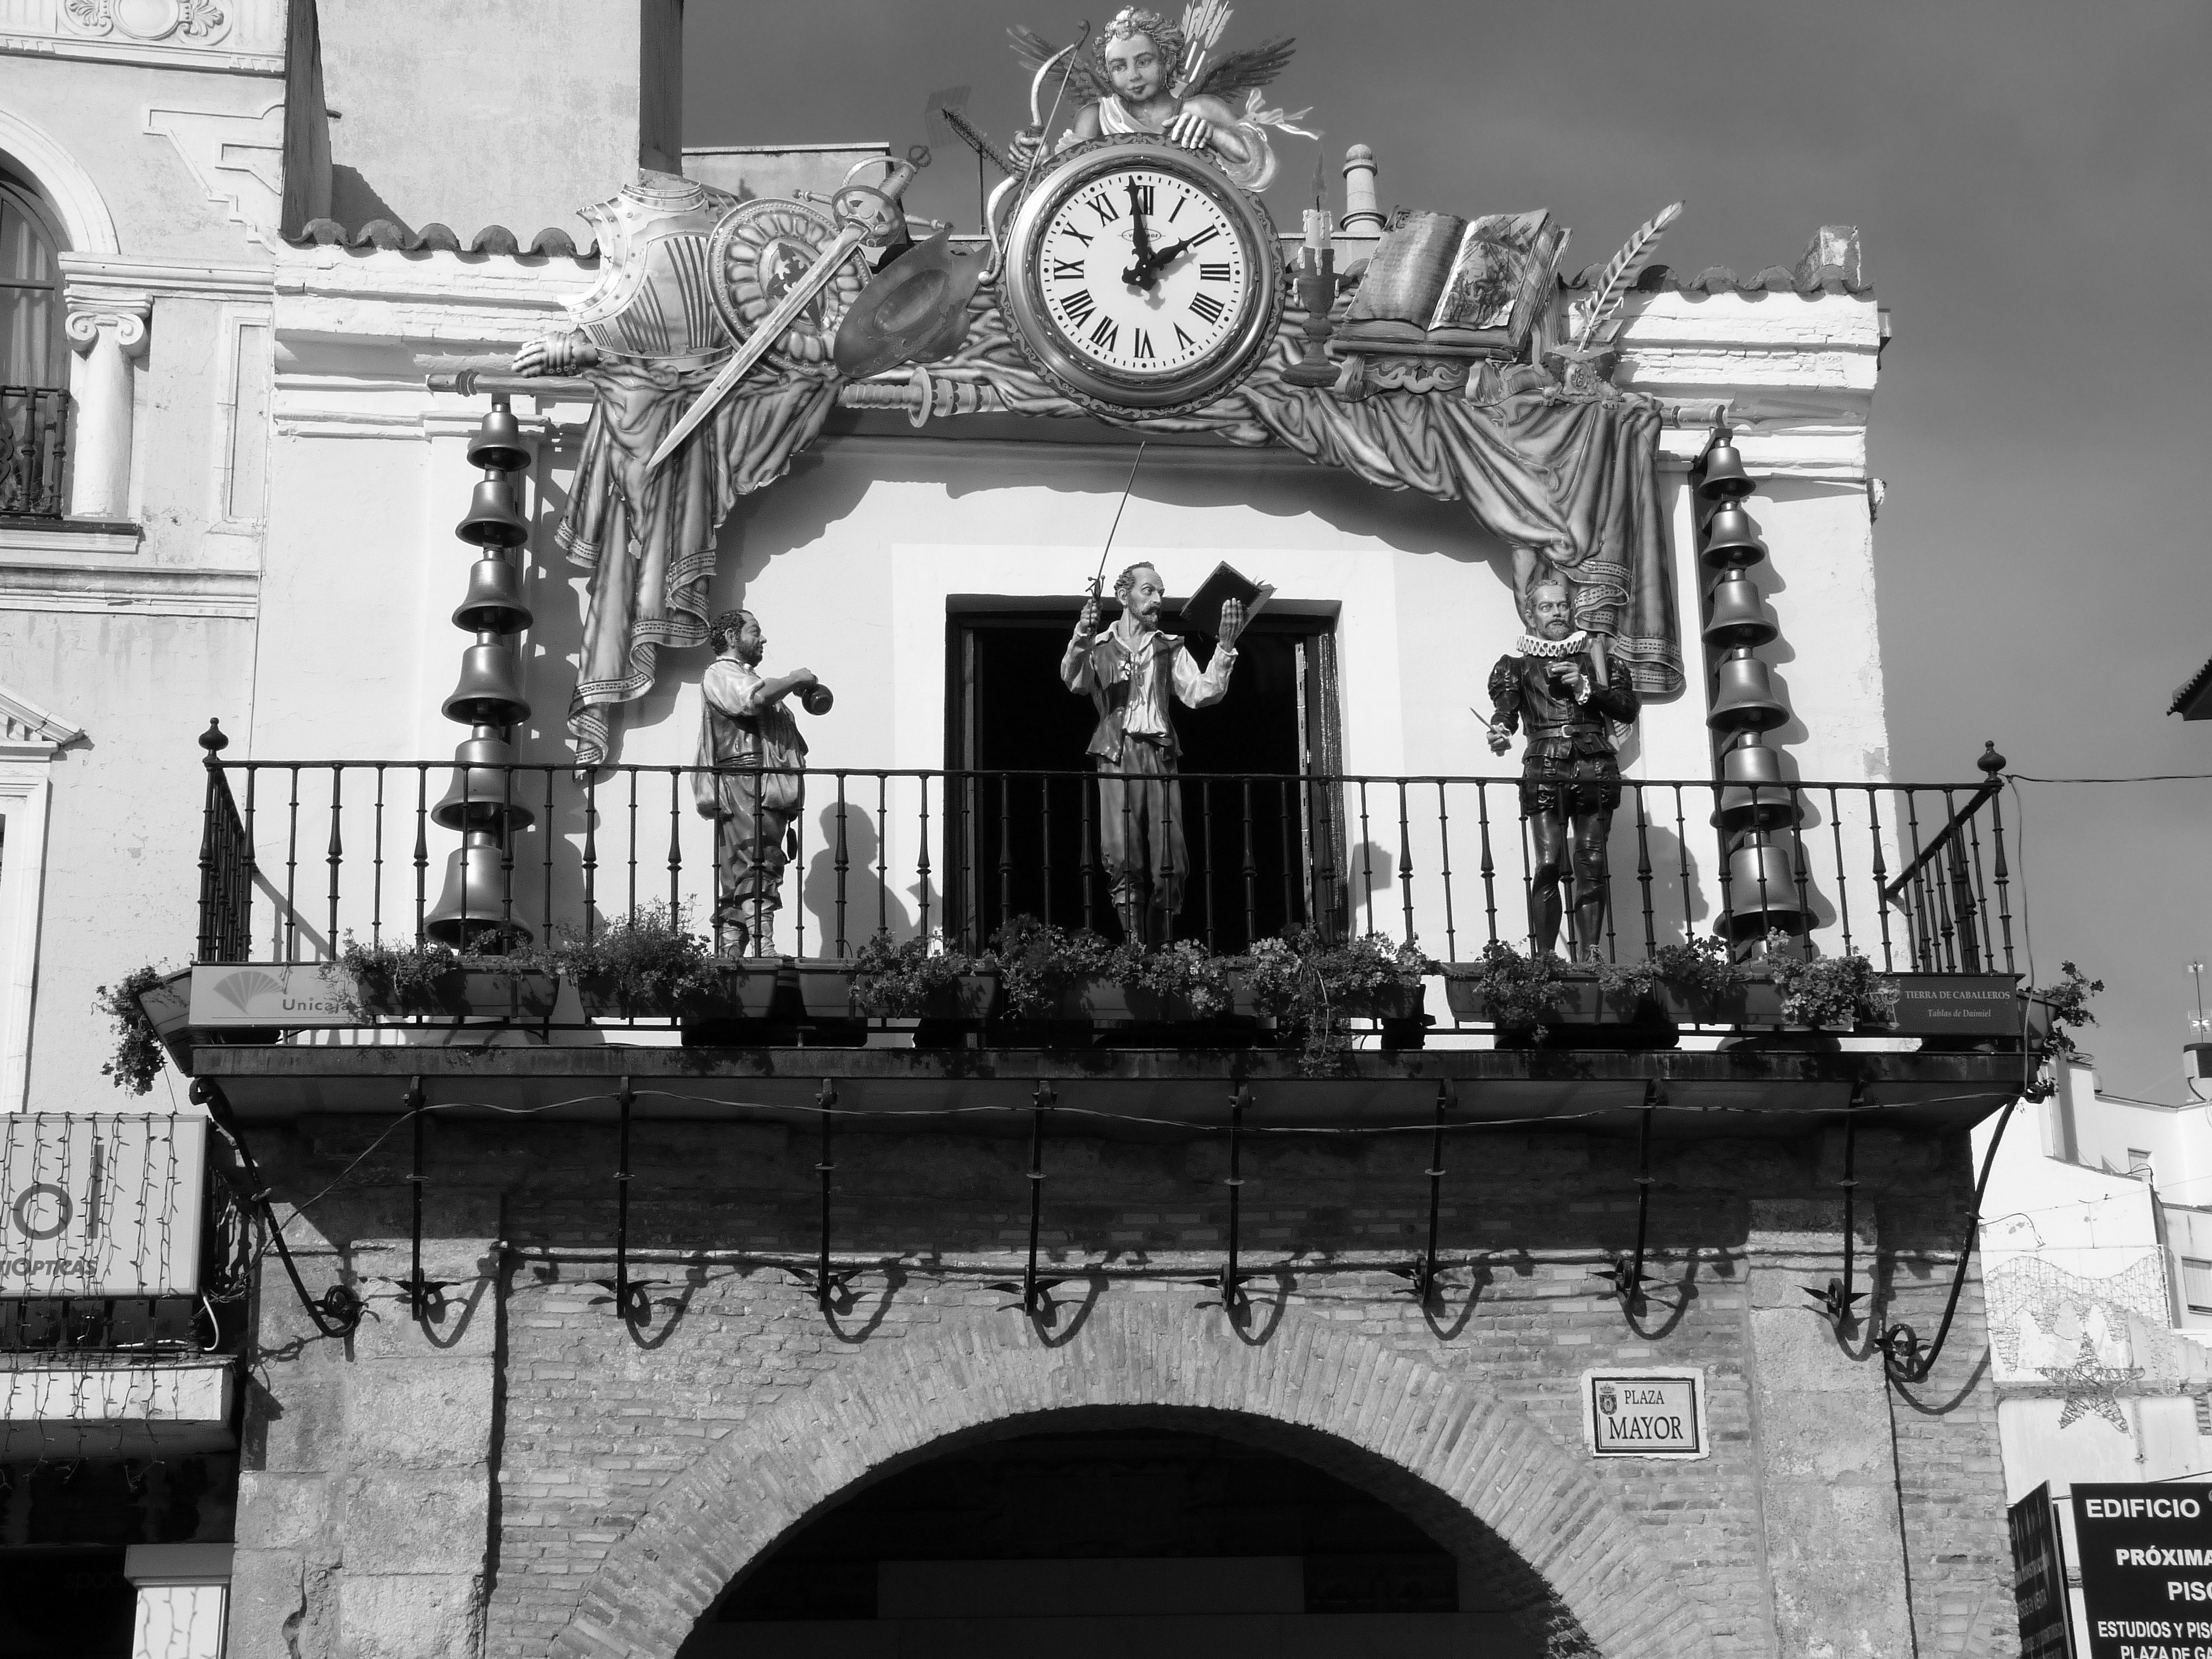
\includegraphics[width=0.8\linewidth]{./figs/clockCRbw}
		\caption{Fotografía en blanco y negro}\label{fig:fotoBW}
	\end{subfigure} 
	\caption[Ejemplo de subfiguras]{Ejemplo de inclusión de subfiguras en un mismo entorno (Fuente: J. Salido, \faCreativeCommons{} \faCreativeCommonsBy{} \faCreativeCommonsNcEu{} \faCreativeCommonsNd)}
	\label{fig:ejSubfigures}
\end{figure}

En los trabajos académicos la inclusión de imágenes y figuras que no son propiedad del autor suscitan bastante controversia, ya que con frecuencia se incumple inadvertidamente la ley vigente de propiedad intelectual. Respecto a este hecho se recomienda, tanto a estudiantes como tutores, consultar documentación informativa sobre el uso correcto de figuras en documentos académicos \cite{uclm20,unican18}. Entre las <<incorrecciones>> más habituales en los documentos académicos, se observa:
\begin{itemize}
\item \emph{Abuso del derecho de cita}. Se produce al incluir, con fines exclusivamente decorativos o ilustrativos de la explicación, una figura sujeta a derechos de uso restringido invocando el derecho de cita (incluso con correcta atribución de la obra).

\item \emph{Incorrecta atribución de la obra}. Es habitual confundir al autor de la obra con la fuente de origen de la misma. La fuente es precisa cuando se cita la obra original. Sin embargo, la licencia de muchas obras exige la atribución al autor y la inclusión de la licencia bajo la que se distribuye o hace uso de la misma (véase como ejemplo cómo se realiza una correcta atribución en las Fig.~\ref{fig:ejFigure} y \ref{fig:ejSubfigures} mencionando al autor y la licencia Creative-Commons\footnote{\url{https://creativecommons.org}} bajo la que se rige el uso de la imagen y el mecanismo de título alternativo para que dicha atribución no aparezca en el índice de figuras usando título opcional).

\item \emph{Supresión de los detalles de la licencia de uso}. Al incluir obras de terceros debemos tener presente los términos de distribución de la misma e incluirlos junto a la atribución de su legítimo autor.
\end{itemize}

La inclusión de material de \emph{dominio público}, sin restricciones de uso o con permiso, hace innecesaria la atribución al autor, pero se recomienda incluir una nota de agradecimiento.\footnote{Incluyendo un texto como: \emph{<<Por cortesía de ...>>}}

Cuando se presenta la necesidad de incluir un gráfico demasiado grande para el tamaño de la página, una opción muy apropiada es la impresión del gráfico en modo girado en una página aparte. Este efecto se consigue con el entorno \texttt{sidewaysfigure} proporcionado por el paquete \texttt{rotating}. La Fig.~\ref{fig:girada} muestra un ejemplo del entorno citado con un gráfico \textsf{PDF}.

\begin{sidewaysfigure}
	\centering
	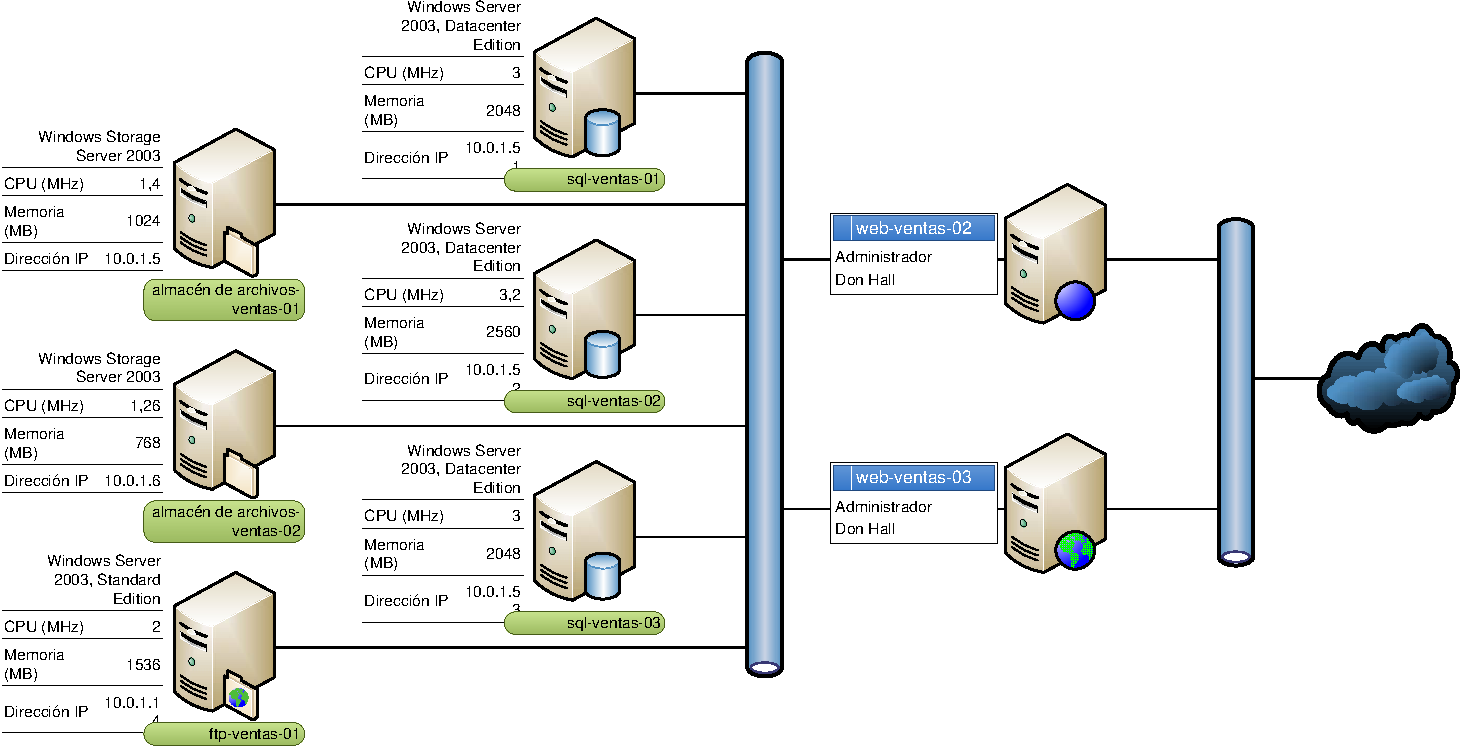
\includegraphics[width=0.98\textheight]{./figs/network} 
	\caption[Gráfico girado]{Figura vectorial con impresión girada}
	\label{fig:girada}
\end{sidewaysfigure}


\begin{landscape}
\thispagestyle{empty}
También es posible imprimir una página en formato apaisado cuando contiene una figura muy ancha. Este efecto se consigue con el paquete \texttt{pdflscape} y el entorno \texttt{landscape} proporcionado. Además, es este caso se han suprimido tanto la cabecera como el pie de página. La figura~\ref{fig:apaisada} se muestra apaisada a modo de ejemplo.

\begin{figure}[H]
	\centering
	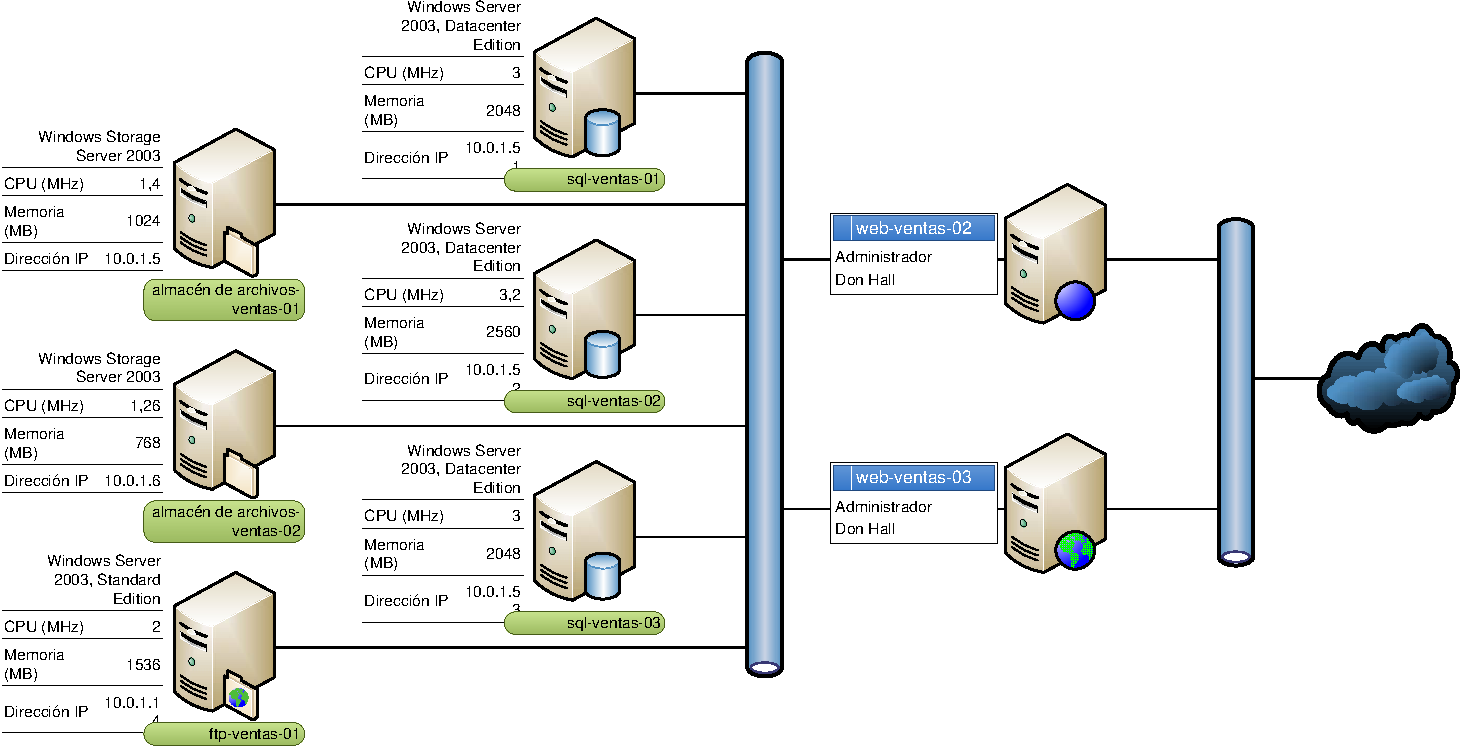
\includegraphics[width=\linewidth]{./figs/network} 
	\caption[Gráfico apaisado]{Figura vectorial con vista en página apaisada}
	\label{fig:apaisada}
\end{figure}
\end{landscape}


\section{Algoritmos y listados de código fuente}
En los textos científicos relacionados con las 
TIC\footnote{Por supuesto, en un TFG (Trabajo Fin de Grado) o tesis 
de un centro superior de Informática.} (Tecnologías de la Información y 
Comunicaciones) suelen aparecer porciones de código en los que se explica 
alguna función o característica relevante del trabajo que se expone. Muchas 
veces lo que se quiere ilustrar es un algoritmo o método con el que se resuelve un problema abstrayéndose del lenguaje de implementación. El paquete \texttt{algorithm2e} proporciona un entorno \texttt{algorithm} para la impresión apropiada de algoritmos, tratándolos como objetos flotantes y con mucha flexibilidad de personalización, como se observa en el algoritmo~\ref{alg:como} del ejemplo.


% Ejemplo:
% ============
\IncMargin{1em}
\begin{algorithm}
\SetKwInOut{Input}{Datos}\SetKwInOut{Output}{Resultado}
\LinesNumbered
\SetAlgoLined

\Input{este texto} 
%\KwIn{este texto}
\Output{como escribir algoritmos con \LaTeX2e}
%\KwOut{como escribir algoritmos con \LaTeX2e}

inicialización\;
\While{no es el fin del documento}{
	leer actual\;
	\eIf{comprendido}{
		ir a la siguiente sección\;
		la sección actual es esta\;
	}{
		ir al principio de la sección actual\;
	}
}

% Aunque el captión aparece abajo siempre se pone arriba como en tablas y listados
\caption{Cómo escribir algoritmos}\label{alg:como}
\end{algorithm}\DecMargin{1em}








\newpage % Añadido para visualizar los listados completos en una página.
La inclusión de porciones de código fuente se puede formatear de modo sencillo en \LaTeX{} mediante el uso del paquete \texttt{listings}. A continuación, se muestran varios ejemplos de porciones de código correspondientes a distintos lenguajes de programación.


% Ejemplo: Listado Java
% ============
% Los entornos lstlisting se pueden tratar tambión como elementos flotantes mediante la opción 'float=hbt', donde se indica la ubicación del elemento.
\begin{lstlisting}[language=Java,caption={[Código fuente en Java]Ejemplo de código fuente en lenguaje Java},label=lst:java]
// @author www.javadb.com
public class Main {    
// Este método convierte un String a un vector de bytes

public void convertStringToByteArray() {

String stringToConvert = "This String is 15";      
	byte[] theByteArray = stringToConvert.getBytes();        
	System.out.println(theByteArray.length);        
}

public static void main(String[] args) {
	new Main().convertStringToByteArray();
}
}
\end{lstlisting}


\begin{lstlisting}[style=ruled,language=C,caption={Ejemplo de código fuente en lenguaje C},label=lst:codC]
// Este código se ha incluido tal cual está en el fichero \LaTeX{}
#include <stdio.h>

int main(int argc, char* argv[]) {
	puts("¡Hola mundo!");
}
\end{lstlisting}


\begin{lstlisting}[style=ruled,language=Matlab,caption={Ejemplo de script en Matlab},label=lst:matlab]
function f = fibonacci(n)
% FIBONACCI  Fibonacci sequence
% f = FIBONACCI(n) generates the first n Fibonacci numbers.
%   Copyright 2014 Cleve Moler
% 	Copyright 2014 The MathWorks, Inc.

	f = zeros(n,1); 
	f(1) = 1;
	f(2) = 2;
	for k = 3:n
		f(k) = f(k-1) + f(k-2);
end
\end{lstlisting}



\section{Menús, paths y teclas con el paquete \texttt{menukeys}}
Cada vez es más usual que los trabajos en ingeniería exijan el uso de 
software. Para poder especificar de modo elegante el uso de menús, pulsaciones de teclas y directorios, se recomienda el uso del paquete 
\texttt{menukeys}.\footnote{\url{https://osl.ugr.es/CTAN/macros/latex/contrib/menukeys/menukeys.pdf}}
 \index{CTAN} Este paquete nos permite especificar el acceso a un menú, por 
ejemplo:

\noindent \menu{Herramientas:Órdenes:PDFLaTeX}

\noindent También un conjunto de teclas. Por ejemplo:
\keys{\ctrl + \shift + T}

\noindent O un directorio:
\directory{C:/user/LaTeX/Ejemplos}

\noindent Aunque este paquete permite muchas opciones de configuración de los estilos aplicados, esto no es necesario para obtener unos resultados muy elegantes.










 % Apéndice A (opcionales)
%--- (FIN DOCUMENTO)
\end{document}